\documentclass[10.5pt]{article}
\usepackage[utf8]{inputenc}\usepackage[T1]{fontenc}
\usepackage{amsmath,amsthm,amssymb,enumitem,booktabs,xcolor,tikz,longtable,array,needspace,graphicx}
\usepackage{geometry}
\newcommand{\sect}[1]{\par\medskip\noindent\textbf{\large #1}\par\smallskip}
\theoremstyle{definition}\newtheorem*{example}{Example}\newtheorem*{method*}{Method}
\theoremstyle{remark}\newtheorem*{remark}{Remark}

\newcommand{\chili}{\tikz[baseline=-0.25ex,scale=0.5]{\fill[red!80!black](0,0.12)..controls(0.3,0.16)and(0.55,0.0)..(0.66,-0.22)..controls(0.42,-0.07)and(0.2,-0.04)..(0,-0.1)--cycle;\fill[green!45!black](-0.04,-0.02)rectangle(0.04,0.16);}}
\newcommand{\spice}[1]{\foreach\i in {1,...,#1}{\chili\,}}
\geometry{letterpaper,margin=0.8in}\setlength{\parindent}{0pt}\setlength{\parskip}{0.3em}

\begin{document}

{\Large\textbf{Slot 14 problem sheet: the table as a map of configurations}}\par

\textit{Work in your notebook, numbered, one answer under another. No answer space here. Predict in words before you calculate. On a 3 or 4 chili problem, write what you tried first; then you may ask for a nudge.}\par

\textit{Spice: \spice{1} one step, \spice{2} two steps or an explanation, \spice{3} a graph, two steps or an argument, \spice{4} a hidden quantity.}\par

\begin{center}
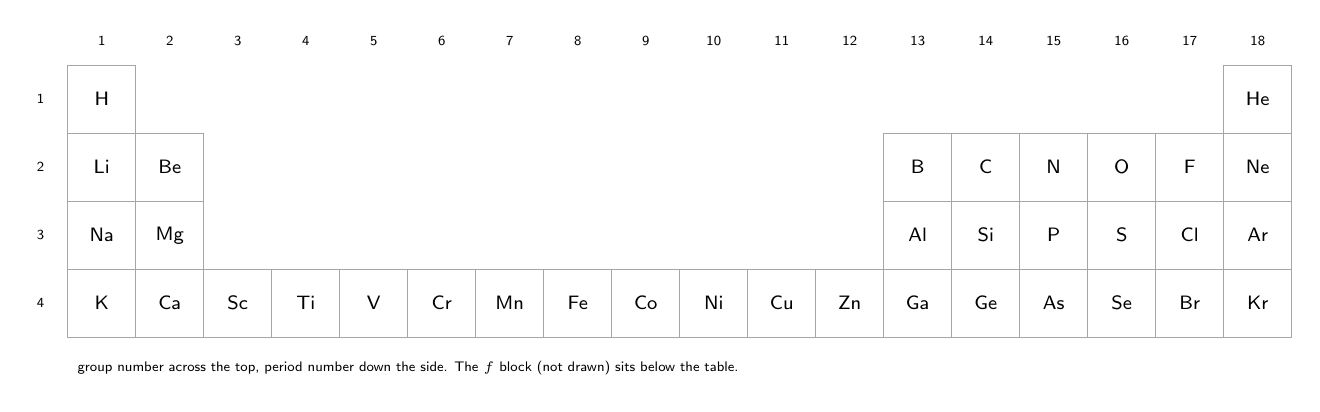
\begin{tikzpicture}[x=0.34in,y=-0.34in,every node/.style={font=\scriptsize\sffamily}]
\node[font=\tiny\sffamily] at (0.50,-0.35) {1};
\node[font=\tiny\sffamily] at (1.50,-0.35) {2};
\node[font=\tiny\sffamily] at (2.50,-0.35) {3};
\node[font=\tiny\sffamily] at (3.50,-0.35) {4};
\node[font=\tiny\sffamily] at (4.50,-0.35) {5};
\node[font=\tiny\sffamily] at (5.50,-0.35) {6};
\node[font=\tiny\sffamily] at (6.50,-0.35) {7};
\node[font=\tiny\sffamily] at (7.50,-0.35) {8};
\node[font=\tiny\sffamily] at (8.50,-0.35) {9};
\node[font=\tiny\sffamily] at (9.50,-0.35) {10};
\node[font=\tiny\sffamily] at (10.50,-0.35) {11};
\node[font=\tiny\sffamily] at (11.50,-0.35) {12};
\node[font=\tiny\sffamily] at (12.50,-0.35) {13};
\node[font=\tiny\sffamily] at (13.50,-0.35) {14};
\node[font=\tiny\sffamily] at (14.50,-0.35) {15};
\node[font=\tiny\sffamily] at (15.50,-0.35) {16};
\node[font=\tiny\sffamily] at (16.50,-0.35) {17};
\node[font=\tiny\sffamily] at (17.50,-0.35) {18};
\node[font=\tiny\sffamily] at (-0.4,0.50) {1};
\node[font=\tiny\sffamily] at (-0.4,1.50) {2};
\node[font=\tiny\sffamily] at (-0.4,2.50) {3};
\node[font=\tiny\sffamily] at (-0.4,3.50) {4};
\draw[gray!70,line width=0.3pt] (0,0) rectangle (1,1);
\node at (0.50,0.50) {H};
\draw[gray!70,line width=0.3pt] (17,0) rectangle (18,1);
\node at (17.50,0.50) {He};
\draw[gray!70,line width=0.3pt] (0,1) rectangle (1,2);
\node at (0.50,1.50) {Li};
\draw[gray!70,line width=0.3pt] (1,1) rectangle (2,2);
\node at (1.50,1.50) {Be};
\draw[gray!70,line width=0.3pt] (12,1) rectangle (13,2);
\node at (12.50,1.50) {B};
\draw[gray!70,line width=0.3pt] (13,1) rectangle (14,2);
\node at (13.50,1.50) {C};
\draw[gray!70,line width=0.3pt] (14,1) rectangle (15,2);
\node at (14.50,1.50) {N};
\draw[gray!70,line width=0.3pt] (15,1) rectangle (16,2);
\node at (15.50,1.50) {O};
\draw[gray!70,line width=0.3pt] (16,1) rectangle (17,2);
\node at (16.50,1.50) {F};
\draw[gray!70,line width=0.3pt] (17,1) rectangle (18,2);
\node at (17.50,1.50) {Ne};
\draw[gray!70,line width=0.3pt] (0,2) rectangle (1,3);
\node at (0.50,2.50) {Na};
\draw[gray!70,line width=0.3pt] (1,2) rectangle (2,3);
\node at (1.50,2.50) {Mg};
\draw[gray!70,line width=0.3pt] (12,2) rectangle (13,3);
\node at (12.50,2.50) {Al};
\draw[gray!70,line width=0.3pt] (13,2) rectangle (14,3);
\node at (13.50,2.50) {Si};
\draw[gray!70,line width=0.3pt] (14,2) rectangle (15,3);
\node at (14.50,2.50) {P};
\draw[gray!70,line width=0.3pt] (15,2) rectangle (16,3);
\node at (15.50,2.50) {S};
\draw[gray!70,line width=0.3pt] (16,2) rectangle (17,3);
\node at (16.50,2.50) {Cl};
\draw[gray!70,line width=0.3pt] (17,2) rectangle (18,3);
\node at (17.50,2.50) {Ar};
\draw[gray!70,line width=0.3pt] (0,3) rectangle (1,4);
\node at (0.50,3.50) {K};
\draw[gray!70,line width=0.3pt] (1,3) rectangle (2,4);
\node at (1.50,3.50) {Ca};
\draw[gray!70,line width=0.3pt] (2,3) rectangle (3,4);
\node at (2.50,3.50) {Sc};
\draw[gray!70,line width=0.3pt] (3,3) rectangle (4,4);
\node at (3.50,3.50) {Ti};
\draw[gray!70,line width=0.3pt] (4,3) rectangle (5,4);
\node at (4.50,3.50) {V};
\draw[gray!70,line width=0.3pt] (5,3) rectangle (6,4);
\node at (5.50,3.50) {Cr};
\draw[gray!70,line width=0.3pt] (6,3) rectangle (7,4);
\node at (6.50,3.50) {Mn};
\draw[gray!70,line width=0.3pt] (7,3) rectangle (8,4);
\node at (7.50,3.50) {Fe};
\draw[gray!70,line width=0.3pt] (8,3) rectangle (9,4);
\node at (8.50,3.50) {Co};
\draw[gray!70,line width=0.3pt] (9,3) rectangle (10,4);
\node at (9.50,3.50) {Ni};
\draw[gray!70,line width=0.3pt] (10,3) rectangle (11,4);
\node at (10.50,3.50) {Cu};
\draw[gray!70,line width=0.3pt] (11,3) rectangle (12,4);
\node at (11.50,3.50) {Zn};
\draw[gray!70,line width=0.3pt] (12,3) rectangle (13,4);
\node at (12.50,3.50) {Ga};
\draw[gray!70,line width=0.3pt] (13,3) rectangle (14,4);
\node at (13.50,3.50) {Ge};
\draw[gray!70,line width=0.3pt] (14,3) rectangle (15,4);
\node at (14.50,3.50) {As};
\draw[gray!70,line width=0.3pt] (15,3) rectangle (16,4);
\node at (15.50,3.50) {Se};
\draw[gray!70,line width=0.3pt] (16,3) rectangle (17,4);
\node at (16.50,3.50) {Br};
\draw[gray!70,line width=0.3pt] (17,3) rectangle (18,4);
\node at (17.50,3.50) {Kr};
\node[font=\tiny\sffamily,anchor=west] at (0,4.45) {group number across the top, period number down the side. The $f$ block (not drawn) sits below the table.};
\end{tikzpicture}
\end{center}

\sect{Review (L1 to L4)}

\noindent\hangindent=7em\hangafter=1\makebox[7em][l]{\textbf{L1}}Write the full configuration of lithium (Z = 3).\par\smallskip

\noindent\hangindent=7em\hangafter=1\makebox[7em][l]{\textbf{L2}}Write the full configuration of sodium (Z = 11).\par\smallskip

\noindent\hangindent=7em\hangafter=1\makebox[7em][l]{\textbf{L3}}Lithium and sodium are in the same group. What do the last pieces of their configurations have in common?\par\smallskip

\noindent\hangindent=7em\hangafter=1\makebox[7em][l]{\textbf{L4}}Guess, no penalty: how many elements are in the fourth row of the periodic table?\par\smallskip

\sect{Conceptual questions}

\textit{C1 to C3 we do together at the board. Do C4 to C6 on your own.}\par

\needspace{4\baselineskip}\noindent\hangindent=7em\hangafter=1\makebox[7em][l]{\textbf{C1}\ \spice{2}}Period 3 has 8 elements and period 4 has 18. What does period 4 have that period 3 does not?\par\medskip

\needspace{4\baselineskip}\noindent\hangindent=7em\hangafter=1\makebox[7em][l]{\textbf{C2}\ \spice{1}}Which block are potassium, iron and gallium in?\par\medskip

\needspace{4\baselineskip}\noindent\hangindent=7em\hangafter=1\makebox[7em][l]{\textbf{C3}\ \spice{2}}Chlorine is in group 17. Write its valence configuration and count its valence electrons.\par\medskip

\needspace{4\baselineskip}\noindent\hangindent=7em\hangafter=1\makebox[7em][l]{\textbf{C4}\ \spice{2}}Think and rank. Without looking at the table, rank these atoms from the fewest valence electrons to the most: (A) chlorine, (B) magnesium, (C) aluminum, (D) argon. Then check on the table.\par\medskip

\needspace{4\baselineskip}\noindent\hangindent=7em\hangafter=1\makebox[7em][l]{\textbf{C5}\ \spice{2}}A student says: ``Every atom in group 18 has 8 valence electrons.'' When is that true, and when is it not?\par\medskip

\needspace{4\baselineskip}\noindent\hangindent=7em\hangafter=1\makebox[7em][l]{\textbf{C6}\ \spice{2}}A student writes: ``Arsenic is in period 4, group 15, so it is $4s^{2}3d^{3}$.'' Find the error and fix it.\par\medskip

\sect{Practice}\textit{Core: C4 to C6 and P1 to P5. Then the rest.}\par

\needspace{4\baselineskip}\noindent\hangindent=7em\hangafter=1\makebox[7em][l]{\textbf{P1}\ \spice{1}}On the table above, shade the $s$ block, the $p$ block and the $d$ block with three different patterns. Write the period number beside each row. Mark with an arrow where the $f$ block would sit.\par\medskip

\needspace{4\baselineskip}\noindent\hangindent=7em\hangafter=1\makebox[7em][l]{\textbf{P2}\ \spice{1}}Give the block, period and group of (a) magnesium (Z = 12), (b) chlorine (Z = 17), (c) iron (Z = 26). Read them off the table.\par\medskip

\needspace{4\baselineskip}\noindent\hangindent=7em\hangafter=1\makebox[7em][l]{\textbf{P3}\ \spice{1}}Write the valence configuration, with no full configuration, for the element in (a) period 2, group 2; (b) period 3, group 13; (c) period 3, group 15.\par\medskip

\needspace{4\baselineskip}\noindent\hangindent=7em\hangafter=1\makebox[7em][l]{\textbf{P4}\ \spice{2}}Which element has the valence configuration (a) $3s^{1}$? (b) $4s^{2}4p^{2}$? Give its period and group.\par\medskip

\needspace{4\baselineskip}\noindent\hangindent=7em\hangafter=1\makebox[7em][l]{\textbf{P5}\ \spice{2}}An atom's full configuration is $1s^{2}2s^{2}2p^{6}3s^{2}3p^{6}4s^{2}3d^{8}$. Add up the electrons to find Z, then give the element, block, period and group.\par\medskip

\needspace{4\baselineskip}\noindent\hangindent=7em\hangafter=1\makebox[7em][l]{\textbf{P6}\ \spice{2}}Give the block, period and group of (a) potassium (Z = 19), (b) gallium (Z = 31), (c) krypton (Z = 36). Then write the valence configuration of (b) and (c).\par\medskip

\needspace{4\baselineskip}\noindent\hangindent=7em\hangafter=1\makebox[7em][l]{\textbf{P7}\ \spice{1}}Which element has the valence configuration (a) $2s^{2}2p^{4}$? (b) $4s^{2}4p^{5}$? How many valence electrons does each have?\par\medskip

\needspace{4\baselineskip}\noindent\hangindent=7em\hangafter=1\makebox[7em][l]{\textbf{P8}\ \spice{2}}An element is in period 4, the $d$ block, group 7. Name it and give its atomic number.\par\medskip

\needspace{4\baselineskip}\noindent\hangindent=7em\hangafter=1\makebox[7em][l]{\textbf{P9}\ \spice{2}}Which element in period 3 has 3 valence electrons? Which has 5? Which has 7?\par\medskip

\sect{Challenge}

\needspace{4\baselineskip}\noindent\hangindent=7em\hangafter=1\makebox[7em][l]{\textbf{H1}\ \spice{3}}The graph shows the number of valence electrons for every atom from $Z=3$ to $Z=18$.\par\medskip
\begin{center}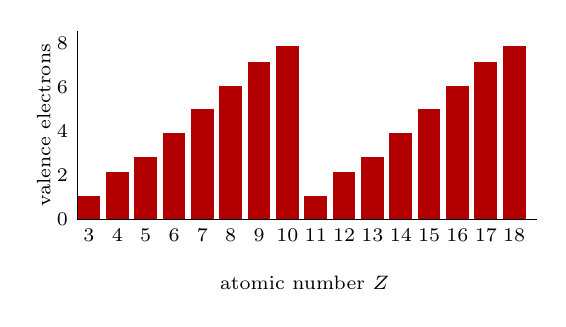
\begin{tikzpicture}[x=0.36cm]\fill[red!70!black] (0,0) rectangle (0.8,0.3);\fill[red!70!black] (1,0) rectangle (1.8,0.6);\fill[red!70!black] (2,0) rectangle (2.8,0.8);\fill[red!70!black] (3,0) rectangle (3.8,1.1);\fill[red!70!black] (4,0) rectangle (4.8,1.4);\fill[red!70!black] (5,0) rectangle (5.8,1.7);\fill[red!70!black] (6,0) rectangle (6.8,2.0);\fill[red!70!black] (7,0) rectangle (7.8,2.2);\fill[red!70!black] (8,0) rectangle (8.8,0.3);\fill[red!70!black] (9,0) rectangle (9.8,0.6);\fill[red!70!black] (10,0) rectangle (10.8,0.8);\fill[red!70!black] (11,0) rectangle (11.8,1.1);\fill[red!70!black] (12,0) rectangle (12.8,1.4);\fill[red!70!black] (13,0) rectangle (13.8,1.7);\fill[red!70!black] (14,0) rectangle (14.8,2.0);\fill[red!70!black] (15,0) rectangle (15.8,2.2);\draw (0,0)--(16.2,0);\draw (0,0)--(0,2.4);\node[font=\scriptsize,below] at (0.4,0){3};\node[font=\scriptsize,below] at (1.4,0){4};\node[font=\scriptsize,below] at (2.4,0){5};\node[font=\scriptsize,below] at (3.4,0){6};\node[font=\scriptsize,below] at (4.4,0){7};\node[font=\scriptsize,below] at (5.4,0){8};\node[font=\scriptsize,below] at (6.4,0){9};\node[font=\scriptsize,below] at (7.4,0){10};\node[font=\scriptsize,below] at (8.4,0){11};\node[font=\scriptsize,below] at (9.4,0){12};\node[font=\scriptsize,below] at (10.4,0){13};\node[font=\scriptsize,below] at (11.4,0){14};\node[font=\scriptsize,below] at (12.4,0){15};\node[font=\scriptsize,below] at (13.4,0){16};\node[font=\scriptsize,below] at (14.4,0){17};\node[font=\scriptsize,below] at (15.4,0){18};\node[font=\scriptsize,left] at (0,0.00){0};\node[font=\scriptsize,left] at (0,0.56){2};\node[font=\scriptsize,left] at (0,1.12){4};\node[font=\scriptsize,left] at (0,1.68){6};\node[font=\scriptsize,left] at (0,2.24){8};\node[font=\scriptsize] at (8,-0.8){atomic number $Z$};\node[font=\scriptsize,rotate=90] at (-1.2,1.2){valence electrons};\end{tikzpicture}\end{center}(a) At which $Z$ does the graph reach 8, each time? (b) At which $Z$ does it fall back to 1? (c) How many elements are between those two falls? Say what that number means about the shell. (d) Predict the next $Z$ where the graph would show 1, and name the element.\par\medskip

\needspace{4\baselineskip}\noindent\hangindent=7em\hangafter=1\makebox[7em][l]{\textbf{H2}\ \spice{3}}An atom has 34 electrons. Use the filling order to write its full configuration, then give its period, block, group, valence configuration and number of valence electrons.\par\medskip

\needspace{4\baselineskip}\noindent\hangindent=7em\hangafter=1\makebox[7em][l]{\textbf{H3}\ \spice{3}}A student says: ``Chlorine is in group 17, so it has 17 valence electrons.'' Write a reply, in two or three sentences, that corrects the claim and tells the student how to get the right number from the table.\par\medskip

\needspace{4\baselineskip}\noindent\hangindent=7em\hangafter=1\makebox[7em][l]{\textbf{H4}\ \spice{4}}Suppose the filling order were $1s,\ 2s,\ 2p,\ 3s,\ 3p,\ 3d,\ 4s,\ 4p$ (the $3d$ before $4s$). Start a new row each time the outer shell number goes up. How many elements would each of the four rows hold? Explain in one sentence why the real table has rows of 2, 8, 8 and 18 instead.\par\medskip

\par\smallskip{\footnotesize Problems are original, modeled on the style of Hewitt's Conceptual Physics Think and Rank and standard chemistry textbook practice sets.}

\end{document}